\documentclass[a4paper,14pt]{extarticle}

\usepackage[utf8x]{inputenc}
\usepackage[T1,T2A]{fontenc}
\usepackage[russian]{babel}
\usepackage{hyperref}
\usepackage{indentfirst}
\usepackage{here}
\usepackage{array}
\usepackage{graphicx}
\usepackage{caption}
\usepackage{subcaption}
\usepackage{chngcntr}
\usepackage{amsmath}
\usepackage{amssymb}
\usepackage{pgfplots}
\usepackage{pgfplotstable}
\usepackage[left=2cm,right=2cm,top=2cm,bottom=2cm,bindingoffset=0cm]{geometry}
\usepackage{multicol}

\renewcommand{\le}{\ensuremath{\leqslant}}
\renewcommand{\leq}{\ensuremath{\leqslant}}
\renewcommand{\ge}{\ensuremath{\geqslant}}
\renewcommand{\geq}{\ensuremath{\geqslant}}
\renewcommand{\epsilon}{\ensuremath{\varepsilon}}
\renewcommand{\phi}{\ensuremath{\varphi}}

\counterwithin{figure}{section}
\counterwithin{equation}{section}
\counterwithin{table}{section}
\newcommand{\sign}[1][5cm]{\makebox[#1]{\hrulefill}} % Поля подписи и даты
\graphicspath{{pics/}} % Путь до папки с картинками
\captionsetup{justification=centering,margin=1cm}
\def\arraystretch{1.3}

\begin{document}

\begin{titlepage}
\begin{center}
	\textbf{Санкт-Петербургский Политехнический Университет \\Петра Великого}\\[0.3cm]
	\small Институт компьютерных наук и технологий \\[0.3cm]
	\small Кафедра компьютерных систем и программных технологий\\[4cm]
	
	\textbf{ОТЧЕТ}\\ \textbf{о лабораторной работе}\\[0.5cm]
	\textbf{<<Исследование частотных характеристик пассивных RC-цепей>>}\\[0.1cm]
	\textbf{Электротехника и Электроника}\\[10.5cm]
\end{center}

\begin{flushright}
	\begin{minipage}{0.60\textwidth}
		\begin{flushleft}
			\small \textbf{Работу выполнили студенты}\\[3mm]
			\small группа 23501/4 \hspace*{17mm} Дьячков В.В.\\[3mm]
			\small группа 23501/4 \hspace*{17mm} Ламтев А.Ю.\\[5mm]
			
			\small \textbf{Преподаватель}\\[5mm]
		 	\small \sign[3.5cm] \hspace*{8mm} к.т.н., доц. Кочетков Ю.Д.\\[0.5cm]
		\end{flushleft}
	\end{minipage}
\end{flushright}

\vfill

\begin{center}
	\small Санкт-Петербург\\
	\small \the\year
\end{center}
\end{titlepage}

\section{Цель работы}

Овладеть методикой расчета и экспериментально исследовать основные параметры однокаскадных транзисторных усилителей, получить навыки настройки их режимов и снятия частотных характеристик усилителей.

\section{Чертеж схемы исследуемого устройства}

\begin{figure}[H]
	\begin{center}
	\vspace{-0.5cm}
		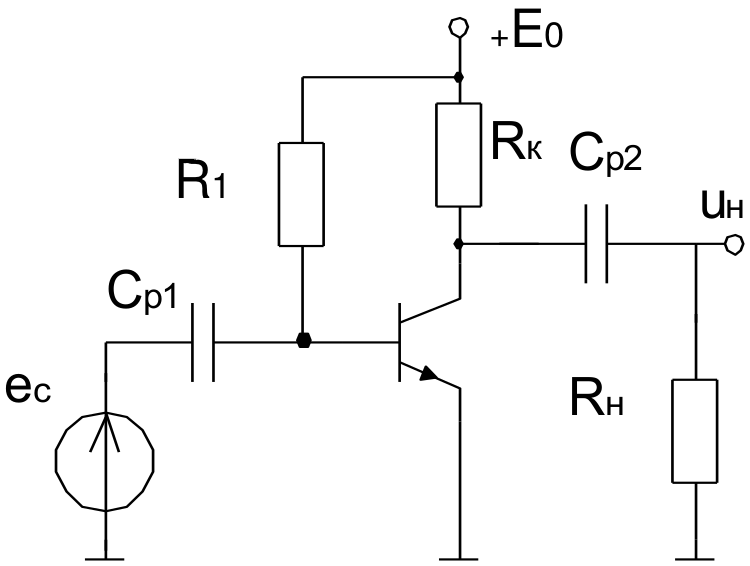
\includegraphics[width=7cm]{img/scheme}
		\caption{Схема однокаскадного усилителя}
		\label{figure:1}
	\vspace{-0.5cm}
	\end{center}
\end{figure}

\section{Исходные данные}

Транзистор МП39. Кремниевый транзистор с $p-n-p$ переходом.

\begin{table}[H]
	\begin{center}
	\caption{Исходные данные}
	\def\arraystretch{1.4}
		\begin{tabularx}{\textwidth}{|X|X|X|X|X|X|X|X|X|X|}
			\hline
			$E_0$ &
			$U_\text{кэА}$ &
			$U_\text{бэ}$ &
			$R_\text{к}$ &
			$R_\text{н}$ &
			$C_{p1}$ &
			$C_{p2}$ &
			$f_{h21}$ &
			$C_\text{к}$ &
			$h_{21}$ \\
			\hline
			В &
			В &
			В &
			кОм &
			кОм &
			мкФ &
			мкФ &
			МГц &
			пФ &
			\\
			\hline
			8 &
			4 &
			0.2 &
			3.9 &
			2 &
			0.22 &
			0.47 &
			0.5 &
			60 &
			12 \\
		    \hline	
		\end{tabularx}
		\label{tabular:1}
	\end{center}
\end{table}

\section{Теоретические расчёты}

Рассчитаем ток эмиттера транзистора: 
\begin{equation}
I_\text{э} = \frac{(E_0 - U_\text{кэА})}{\frac{h_{21}}{1+h_{21}}R_\text{к}} = \frac{8 - 4}{\frac{12}{13} \cdot 3900} = 0.0011 \text{ А}
\end{equation}

Найдем сопротивление резистора $R_1$:
\begin{equation}
R_1 = \frac{h_{21}(E_0-U_\text{БЭ})R_\text{к}}{E_0-U_\text{кэА}} = \frac{12 \cdot (8 - 0.2) \cdot 3900}{4} = 91260 \text{ Ом}
\end{equation}

Рассчитаем входное сопротивление:
\begin{equation}
R_\text{вх} \approx h_\text{11Э} = r_\text{б} + r_\text{э}(h_{21} + 1) = 200 + \frac{0.025}{0.0011} \cdot 13 = 495.45 \text{ Ом}
\end{equation}

Выходное сопротивление примем:
\begin{equation}
R_\text{вых} \approx R_\text{к} = 3.9 \text{ кОм}.
\end{equation}

Найдем коэффициент усиления по току:
\begin{equation}
K_{I0} = h_{21} \cdot \frac{R_1}{R_1 + h_\text{11Э}} \cdot \frac{R_\text{к}}{R_\text{к}+R_\text{н}} 
= 12 \cdot 0.995 \cdot 0.661 = 7.893
\end{equation}

Рассчитаем коэффициент усиления по напряжению:
\begin{equation}
K_{U0} = -\frac{h_{21} R_\text{к} R_\text{н}}{h_\text{11Э}(R_\text{к} + R_\text{н})} = -\frac{12 \cdot 3900 \cdot 2000}{445.45 \cdot 5900} = -35.61
\end{equation}

\newpage

\section{Экспериментально снятые зависимости}

\subsection{Амплитудная характеристика усилителя}

В таблице \ref{tabular:2} приведена амплитудная характеристика усилителя\\ $U_\text{вых} = f(e_c)$. При значениях $e_c > e_{max} = 30.1$ можно заметить искажение входного сигнала. По полученным значениям было вычислено значение коэффициента усиления $K = 55.94$.

\begin{table}[H]
	\begin{center}
	\caption{Зависимость напряжения $U_\text{вых}$ от $e_c$}
	\def\arraystretch{1.2}
		\begin{tabularx}{\textwidth}{|X|X|X|}
			\hline
			$e_c$, мВ & $U_\text{вых}$, мВ & $K$ \\\hline			
			1.43 & 90.1 & 63.01\\\hline	
			3.09 & 200 & 64.72\\\hline	
			5.07 & 324 & 63.91\\\hline	
			7.54 & 476 & 63.13\\\hline	
			10.7 & 675 & 63.08\\\hline	
			13.1 & 799 & 60.99\\\hline	
			15.2 & 913 & 60.07\\\hline	
			17.7 & 1053 & 59.49\\\hline	
			20.7 & 1190 & 57.49\\\hline	
			23.1 & 1310 & 56.71\\\hline	
			25.3 & 1390 & 54.94\\\hline	
			27.9 & 1490 & 53.41\\\hline	
			30.1 & 1580 & 52.49\\\hline\hline
			33.1 & 1690 & 51.06\\\hline	
			35.9 & 1750 & 48.75\\\hline	
			39.6 & 1830 & 46.21\\\hline	
			43.1 & 1910 & 44.32\\\hline	
			45.9 & 1980 & 43.14\\\hline
		\end{tabularx}
		\label{tabular:2}
	\end{center}
\end{table}

\begin{figure}[H]
	\begin{center}
		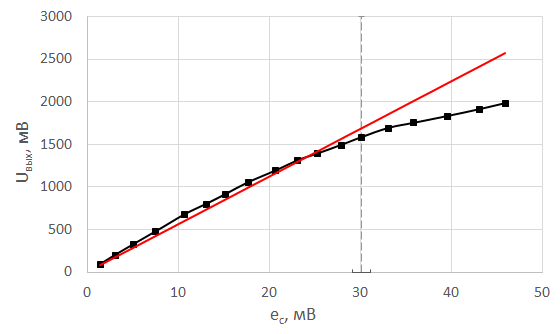
\includegraphics[height=8cm]{img/1}
		\caption{Зависимость напряжения $U_\text{вых}$ от $e_c$}
		\label{figure:2}
	\end{center}
\end{figure}

\subsection{Логарифмическая амплитудно-частотная характеристика усилителя}

В таблице \ref{tabular:3} приведена амплитудно-частотная характеристика усилителя при $e_c = \frac{e_{max}}{2} \approx 20$ мВ.

\begin{table}[H]
	\begin{center}
	\caption{ЛАЧХ усилителя}
	\def\arraystretch{1.2}
		\begin{tabularx}{\textwidth}{|X|X|X|X|}
			\hline
			$f$, Гц & $U_\text{вых}$, В & $K$ & $20 \cdot lg(K)$, дБ\\\hline
			16 & 5.07 & 0.2535 & -11.9204\\\hline
			32 & 17.2 & 0.86 & -1.3100\\\hline
			64 & 49.7 & 2.485 & 7.9065\\\hline
			128 & 119 & 5.95 & 15.4903\\\hline
			256 & 238 & 11.9 & 21.5109\\\hline
			512 & 415 & 20.75 & 26.3404\\\hline
			1024 & 558 & 27.9 & 28.9121\\\hline
			2048 & 623 & 31.15 & 29.8692\\\hline
			4096 & 641 & 32.05 & 30.1166\\\hline
			8192 & 639 & 31.95 & 30.0894\\\hline
			16384 & 621 & 31.05 & 29.8412\\\hline
			32768 & 559 & 27.95 & 28.9276\\\hline
			65536 & 459 & 22.95 & 27.2157\\\hline
			131072 & 353 & 17.65 & 24.9349\\\hline
			200000 & 289 & 14.45 & 23.1974\\\hline
		\end{tabularx}
		\label{tabular:3}
	\end{center}
\end{table}

\begin{figure}[H]
	\begin{center}
		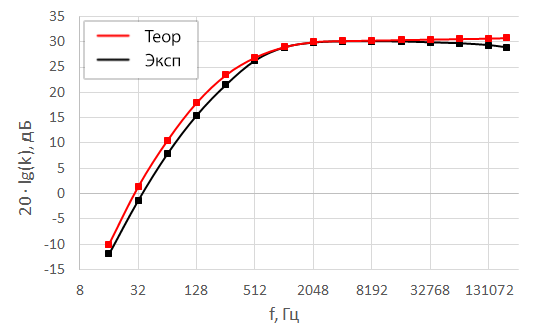
\includegraphics[height=8cm]{img/3}
		\caption{ЛАЧХ усилителя}
		\label{figure:2}
	\end{center}
\end{figure}

\subsection{Измерение входного и выходного сигна}

Для измерения входного сопротивления усилителя последовательно с источником сигнала, был включен измерительный резистор $R_\text{изм} = 680$ Ом, при этом $e_c = 20$ мВ.
\begin{equation}
R_\text{вх} = \frac{U_\text{вх} \cdot R_\text{изм}}{e_c - U_\text{вх}} = \frac{10.1 \cdot 680}{20 - 10.1} = 693.74 \text{ Ом}
\end{equation}

% подгон: слишком много
%\begin{equation}
%R_\text{вх} = \frac{U_\text{вх} \cdot R_\text{изм}}{e_c - U_\text{вх}} = \frac{12.1 \cdot %680}{20 - 12.1} = 1041.5 \text{ Ом}
%\end{equation}

Для измерения выходного сопротивления усилителя, от выхода схемы отключался $R_\text{н}$.
\begin{equation}
R_\text{вых} = \frac{(U_\text{вых хх} - U_\text{вых Rн}) \cdot R_\text{н}}{U_\text{вых Rн}} = \frac{(1.2 - 0.44) \cdot 2000}{0.44} = 3454 \text{ Ом,}
\end{equation}
где $U_\text{вых хх}$ - сопротивление выходного сигнала при отсутствии резистора $R_\text{н}$, $U_\text{вых Rн}$ - сопротивление выходного сигнала при подключенном резисторе $R_\text{н}$.

\section{Уточнение теоретических величин}

На основе проведенного эксперемента были уточнены теоретические значения.

Для получения заданного напряжения $U_\text{кэ} = 4$ В был использован резистор с сопротивлением $R_1 = 80$ (?) кОм. Исходя из этих данные можно рассчитать $h_{21}$:
\begin{equation}
h_{21} = \frac{(E_0 - U_\text{кэА}) \cdot R_1}{R_\text{к}(E_0 - U_\text{бэ})} = \frac{(8 - 4) \cdot ??}{3900 \cdot (8 - 0.2)} = 22.633.
\end{equation}

Так как $h_{11\text{Э}} \simeq R_{\text{вх}} = 693.74$ то можно получить уточненное начение $K_{U0}$: 

\begin{equation*}
K_{U0} = \frac{h_{21}R_\text{н}R_\text{к}}{h_\text{11Э}(R_\text{к}+R_\text{н})} = \frac{? \cdot 3900 \cdot 2000}{693.74 \cdot 5900} = 50.35.
\end{equation*}

Таким образом, 
\begin{equation*}
K_{U0\text{ теор.}} = 40.859 \simeq 41.351 = K_{U0\text{ эксп.}}
\end{equation*}

\section{Анализ погрешностей}

\subsection{Расчет теоретических погрешностей}

\begin{equation*}
\delta R_\text{0вх} = \sqrt{(\delta R_\text{н})^2 + (\delta R_\text{к})^2} = \sqrt{0.01 + 0.01} = 0.14 = 14 \%
\end{equation*}

\begin{equation*}
\delta R_\text{0вых} = 10\%
\end{equation*}

\begin{equation*}
\delta K_0 = \sqrt{(\delta R_\text{н})^2 + (\delta R_\text{к})^2} = \sqrt{0.01 + 0.01} = 0.14 = 14 \%
\end{equation*}

\subsection{Расчет практических погрешностей}
\begin{equation*}
\delta R_\text{вх} = \frac{|R_\text{вх теор} - R_\text{вх пр}|}{R_\text{вх теор}} = \frac{|445.45 - 693.74|}{445.45} = 0.019 = 1.9 \% < \delta R_\text{0вх}
\end{equation*}

\begin{equation*}
\delta R_\text{вых} = \frac{|R_\text{вых теор} - R_\text{вых пр}|}{R_\text{вых теор}} = \frac{|3900 - 3485|}{3900} = 0.106 = 10.6 \% \approx \delta R_\text{0вых}
\end{equation*}

\begin{equation*}
\delta K = \frac{|K_\text{теор} - K_\text{пр}|}{K_\text{теор}} = \frac{|41.23 - 41.68|}{41.23} = 0.011 = 1.1 \% < \delta K_0
\end{equation*}

\section{Выводы}

\end{document}
